\chapter{Tablet Method}
\label{TabletMethodChapter}

\section{Abstract}

A methodology is proposed that allows for experiments of colour constancy to be performed in real and complex environments, in order to better understand colour constancy in the real world. The methodology considered uses a tablet computer to present a spatial version of an achromatic point selection task. 
The key concerns are whether such a methodology can record differences in perceptual white point, present a stable stimulus across disparate environments, and be suitable for naive observers following minimal instruction. On each point, the method is shown to be at moderately successful, with caveats, and suggestions are provided for improvements.
If judged satisfactory, such a methodology could be used to investigate the effect of multiple cues, conflicting cues and cues which cannot easily be reproduced in a controlled in a lab environment.

\section{Introduction}

To further our understanding of colour constancy, investigators have traditionally designed experiments where the number of variables compared to a real-world environment is greatly reduced. This allows investigators to carefully query the impact of any individual variable, or the interplay of a small number of variables. An example may be the `Mondrian' patterns used in a vast number of investigations, most famously used by \citet{land_retinex_1964} (and well described by \citet{hurlbert_colour_1999}) where an observer is presented with a flat and unmoving selection of overlapping coloured rectangles in place of a real scene, or the more recent experiments of \citet{kraft_mechanisms_1999} where objects representing potential colour constancy cues (such as a tin-foil covered cone) were removed from a neutrally coloured box one-by-one in order to probe their relative usefulness.

\begin{figure}[hbp]
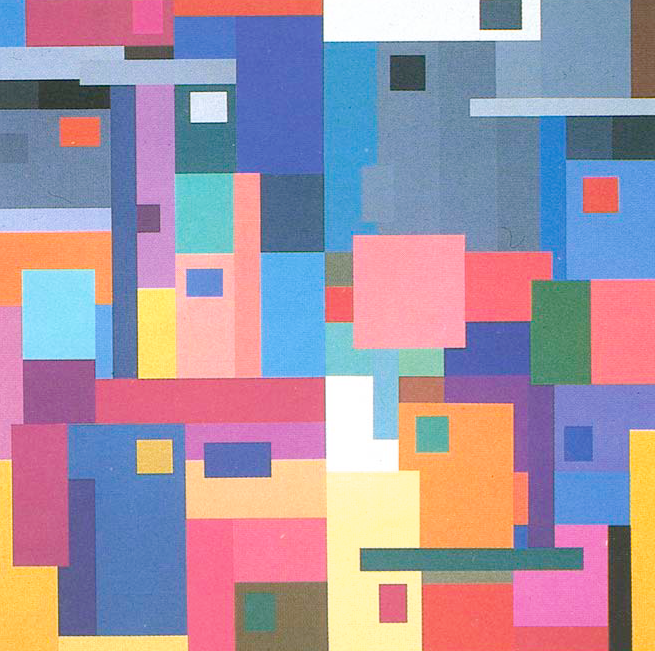
\includegraphics[width=\textwidth]{figs/tablet/mondrian.png}
\caption{An example `Mondrian', reproduced from \citet{land_recent_1986}.}
\label{fig:mondrian}
\end{figure}